\usepackage[paperwidth=105mm,paperheight=297mm,margin=1cm]{geometry}
\usepackage[utf8]{inputenc}
\usepackage[T1]{fontenc}
\usepackage[swedish]{babel}
\usepackage{amsmath}
\usepackage{lmodern}
\usepackage{units}
\usepackage{icomma}
\usepackage{color}
\usepackage{graphicx}
\usepackage{bbm}
\usepackage{hyperref}
\pagenumbering{gobble}
\usepackage{multicol}
\usepackage{titlesec}
\usepackage{mathtools}
\newcommand{\orientation}{\landskap}
%% --- %%

%% Section-format %%
\setlength{\columnsep}{1.5cm}
\titleformat
{\section} % command
[display] % shape
{\bfseries\Large\itshape} % format
{} % label
{0em} % sep
{\vspace{-0.5em}\hspace{-0.05em}} % before-code
[\vspace{0em}] % after-code
\titlespacing{\section}{0em}{0em}{0.2em}
\setlength{\parindent}{0cm}
%% --- %%

%% Titelformat %%
\newcommand{\titelsida}
{
\begin{center}
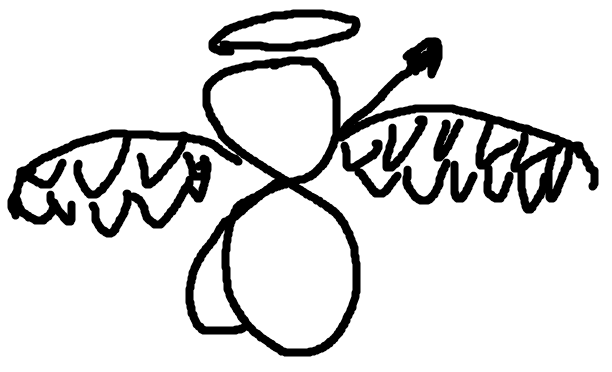
\includegraphics[width=\logga]{logo.png}~\\[0.75em]
{ \Huge \titel \\[0.75em] }
{\large Toastmasters: \host\\[0.5em]}
{\large \datum\\\vspace{0.6em}}
{\large Förrätt: \forratt\\\vspace{0.1em}}
{\large Huvudrätt: \huvudratt\\\vspace{0.1em}}
{\large Efterrätt: \efterratt\\\vspace{0.1em}}
\end{center}
}
%% --- %%

%% Sång %%
\newcommand{\inputsong}[1]{\input{texter/#1.tex}}
%% --- %%

% Environment for songs
\newenvironment{song}[2]{
\section{#1}
\label{#2}
}{}

% Environment for verses
\newenvironment{vers}{
\begin{flushleft}\filbreak
}{
\end{flushleft}{}
}

% Definiera melodirad
\newcommand{\mel}[1]{\begin{flushleft}\textit{\small{Mel: #1}}\end{flushleft}}
% Ta bort eventuella kommentarer i sånghäftet
\newcommand{\av}[1]{}
\newcommand{\kom}[1]{}


% Repriser sheet music
\newcommand{\repopen}
{
	\raisebox{-.4ex}{\rule{.2ex}{2.5ex}\,\rule{.1ex}{2.5ex}}
	\hspace{-0.4ex}\raisebox{.2ex}{:}
}
\newcommand{\repclose}
{
	\raisebox{.2ex}{:}\hspace{-0.4ex}
	\raisebox{-.4ex}{\rule{.1ex}{2.5ex}\,\rule{.2ex}{2.5ex}}
}

% Definiera om sidbrytningar från sjungboken till ingenting - ändra inte
\newcommand{\newp}{}